\documentclass[12pt,]{article}
\usepackage{lmodern}
\usepackage{amssymb,amsmath}
\usepackage{ifxetex,ifluatex}
\usepackage{fixltx2e} % provides \textsubscript
\ifnum 0\ifxetex 1\fi\ifluatex 1\fi=0 % if pdftex
  \usepackage[T1]{fontenc}
  \usepackage[utf8]{inputenc}
\else % if luatex or xelatex
  \ifxetex
    \usepackage{mathspec}
  \else
    \usepackage{fontspec}
  \fi
  \defaultfontfeatures{Ligatures=TeX,Scale=MatchLowercase}
\fi
% use upquote if available, for straight quotes in verbatim environments
\IfFileExists{upquote.sty}{\usepackage{upquote}}{}
% use microtype if available
\IfFileExists{microtype.sty}{%
\usepackage{microtype}
\UseMicrotypeSet[protrusion]{basicmath} % disable protrusion for tt fonts
}{}
\usepackage[margin=1in]{geometry}
\usepackage{hyperref}
\PassOptionsToPackage{usenames,dvipsnames}{color} % color is loaded by hyperref
\hypersetup{unicode=true,
            pdftitle={On the Complexity of Best Arm Identification},
            pdfauthor={Tim Radtke},
            colorlinks=true,
            linkcolor=Maroon,
            citecolor=Blue,
            urlcolor=blue,
            breaklinks=true}
\urlstyle{same}  % don't use monospace font for urls
\usepackage{graphicx,grffile}
\makeatletter
\def\maxwidth{\ifdim\Gin@nat@width>\linewidth\linewidth\else\Gin@nat@width\fi}
\def\maxheight{\ifdim\Gin@nat@height>\textheight\textheight\else\Gin@nat@height\fi}
\makeatother
% Scale images if necessary, so that they will not overflow the page
% margins by default, and it is still possible to overwrite the defaults
% using explicit options in \includegraphics[width, height, ...]{}
\setkeys{Gin}{width=\maxwidth,height=\maxheight,keepaspectratio}
\IfFileExists{parskip.sty}{%
\usepackage{parskip}
}{% else
\setlength{\parindent}{0pt}
\setlength{\parskip}{6pt plus 2pt minus 1pt}
}
\setlength{\emergencystretch}{3em}  % prevent overfull lines
\providecommand{\tightlist}{%
  \setlength{\itemsep}{0pt}\setlength{\parskip}{0pt}}
\setcounter{secnumdepth}{5}
% Redefines (sub)paragraphs to behave more like sections
\ifx\paragraph\undefined\else
\let\oldparagraph\paragraph
\renewcommand{\paragraph}[1]{\oldparagraph{#1}\mbox{}}
\fi
\ifx\subparagraph\undefined\else
\let\oldsubparagraph\subparagraph
\renewcommand{\subparagraph}[1]{\oldsubparagraph{#1}\mbox{}}
\fi

%%% Use protect on footnotes to avoid problems with footnotes in titles
\let\rmarkdownfootnote\footnote%
\def\footnote{\protect\rmarkdownfootnote}

%%% Change title format to be more compact
\usepackage{titling}

% Create subtitle command for use in maketitle
\newcommand{\subtitle}[1]{
  \posttitle{
    \begin{center}\large#1\end{center}
    }
}

\setlength{\droptitle}{-2em}
  \title{On the Complexity of Best Arm Identification}
  \pretitle{\vspace{\droptitle}\centering\huge}
  \posttitle{\par}
  \author{Tim Radtke}
  \preauthor{\centering\large\emph}
  \postauthor{\par}
  \predate{\centering\large\emph}
  \postdate{\par}
  \date{5/20/2017}

\usepackage[retainorgcmds]{IEEEtrantools}
\usepackage{bm}
\usepackage{amsmath}
\usepackage{bbm}
\newtheorem{theorem}{Theorem}
\newtheorem{lemma}{Lemma}
\newcommand{\KL}{\,\text{KL}}
\newcommand{\der}{\,\text{d}}

\begin{document}
\maketitle

In the previous chapter, we have discussed the thresholding bandit
problem as presented in Locatelli et al. (2016). Doing so, we came
across the complexity term \(H = \sum_{i=1}^{K} \Delta_i^{-2}\).
Furthermore, we have noted the fact that an algorithm and bounds based
on \emph{only} the gap between the respective mean and the threshold are
useful in the case of sub-Gaussian problems. Furthermore, even for the
case of Bernoulli arms, which are sub-Gaussian since their feedback is
bounded on \([0,1]\), the gap \(\Delta\) becomes less and less
appropriate for situations in which both \(\mu\) of the Bernoulli, and
\(\tau\) are very close to 0 or 1.

Even though the complexity \(H\) enjoys popularity in the literature of
the best m arm identification problem, \(m \geq 1\), Kaufmann et al.
(2016) show explicitly that \(H\) is mainly useful for problems of
Gaussian distributions. Indeed, they go so far as to define new measures
of complexity that are based on information theoretic metrics. Using
those they then display \(H\) as an approximation to their measures in
the case of Gaussian distributions. In turn, this makes apparent that
especially Bernoulli distributions with small means have to be treated
differently.

For the current chapter, we will adopt the notation of Kaufmann et al.
(2016) so that it will be easier to compare the arguments.

Instead of the thresholding bandit problem, we now consider the problem
of identifying the best \(m\) out of \(K\) arms, that is, the Top-\(m\)
problem. While we previously looked at a fixed budget formulation, we
now mainly focus on a fixed confidence problem. That is, we hold the
confidence \(1-\delta\) fixed at which a strategy returns the correct
\(m\) arms while trying to find them in a way that minimizes the sample
complexity \(\mathbb{E}_{\nu}[\tau]\), that is, the expected number of
overall draws of the arms. \(\tau\) is also called the stopping time of
the algorithm. Algorithms are supposed to find \(\mathcal{S}_m^*\), the
set of the \(m\) arms with the largest means. If we let
\((\mu_1, \dots, \mu_K)\) be the vector of the means of the arms, then
let \((\mu_{[1]}, \dots, \mu_{[K]})\) be the tuple in which the means
are arranged in decreasing order. For the rest of this chapter, we
consider only settings with arms for which \(\mu_{[m]} > \mu_{[m+1]}\);
that is, the set of the top \(m\) arms, \(\mathcal{S}_m^*\), is unique.
After the sampling phase, we require any algorithm to return the set
\(\hat{S}_m \subset \{1,\dots,K\}\) of \(m\) arms that the algorithm
believes to have the largest means. In the case of fixed confidence, we
fix \(\delta\) at the beginning, such that the algorithm only stops
sampling when
\(\mathbb{P}_{\nu}(\hat{S}_m = \mathcal{S}_m^*) \geq 1-\delta\). We try
to find algorithms who fulfill this as quickly as possible; that is,
they minimize the expected stopping time (or number of draws),
\(\mathbb{E}_{\nu}[\tau]\).

To arrive at the new measure of complexity proposed by Kaufmann et al.
(2016), it will actually make sense to first follow their arguments to a
general lower bound on the sample complexity \(\mathbb{E}_{\nu}[\tau]\)
in the case of fixed confidence problems. This bound is given in their
Theorem 4 (for common confidence levels of \(\delta \leq 0.15\)).

\begin{theorem}[Kaufmann et al., 2016] \label{theorem:KaufmannEtAlTheorem4}
Let $\nu \in \mathcal{M}_m$, where $\mathcal{M}_m$ is the set of uniquely identifiable bandit models described above. Assume that $\mathcal{P}$ satisfies the continuity conditions in Assumption 3. Any $\delta$-PAC algorithm on $\mathcal{M}_m$ satisfies, for $\delta \leq 0.15$:

\begin{equation*}
\mathbb{E}_{\nu}[\tau] \geq \Big[ \sum_{a \in \mathcal{S}^*_m} \frac{1}{KL(\nu_a, \nu_{[m+1]})} + \sum_{a \notin \mathcal{S}^*_m} \frac{1}{KL(\nu_a, \nu_{[m]})} \Big] \der(1-\delta, \delta),
\end{equation*}

where $\der(x,y) := x \log(x/y) + (1-x) \log((1-x)/(1-y))$ is the binary relative entropy, with the convention that $\der(0,0) = \der(1,1) = 0$.
\end{theorem}

To proof this statement, we assume as before that the arms are ordered
by their means decreasing in size. For a given \(\delta\)-PAC algorithm
\(\mathcal{A} = ((A_t), \tau, \hat{S}_m)\), and under the continuity
conditions, there exists for every arm \(a \in \{1, \dots, K\}\) an
alternative model
\(\nu' = (\nu_1, \dots, \nu_{a-1}, \nu_a', \nu_{a+1}, \dots, \nu_K)\).
In this alternative model, only arm \(a\) is modified in accordance with
the continuity conditions. Modified in such a way that measured by the
Kullback-Leibler divergence, the arm \(\nu_{m+1}\) is now closer to
\(\nu_a\) than \(\nu_a'\) is to \(\nu_a\), if \(\mu_a > \mu_{m+1}\)
(consequently, \(\mu_a' < \mu_{m+1}\)). On the other hand, if
\(\mu_a < \mu_{m}\), then \(\nu_a'\) will be moved away from \(\nu_a\)
just enough so that \(\nu_a\) is closer to \(\nu_m\) than to \(\nu_a'\)
(consequently, \(\mu_a' > \mu_m\)). These changes in distribution make
the original set of optimal arms, \(\{1,\dots,m\}\) no longer optimal
under the alternative model \(\nu'\). Given that the algorithm returns
\(\hat{S}_m\), we know that for the event
\(\mathcal{E} = (\hat{S}_m = \{1, \dots, m\})\) (which is element of the
by the stopping time \(\tau\) induced \(\sigma\)-Algebra
\(\mathcal{F}_{\tau}\)), that
\(\mathbb{P}_{\nu}(\mathcal{E}) \geq 1-\delta\) and
\(\mathbb{P}_{\nu'}(\mathcal{E}) \leq \delta\) (because fixed confidence
\(\delta\)!).

To now give the lower bound on the expected number of samples,
\(\mathbb{E}_{\nu}[\tau]\), we employ the general lemma given by the
authors for such changes in distribution in bandit models.

\begin{lemma}[Kaufmann et al., 2016] \label{theorem:KaufmannEtAlLemma1}
Let $\nu$ and $\nu'$ be two bandit models with $K$ arms such that for all $a$, the distributions $\nu_a$ and $\nu_a'$ are mutually absolutely continuous. For any almost-surely finite stopping time $\sigma$ with respect to $(\mathcal{F}_t)$,

\begin{equation*}
\sum_{a=1}^{K} \mathbb{E}_{\nu} [N_a(\sigma)] \KL(\nu_a, \nu_a') \geq \sup_{\mathcal{E} \in \mathcal{F}_{\sigma}} \der (\mathbb{P}_{\nu}(\mathcal{E}), \mathbb{P}_{\nu'}(\mathcal{E})),
\end{equation*}

where $\der(x,y)$ is the binary relative entropy as defined above.
\end{lemma}

We can apply this lemma directly on the expected number of draws for
each arm, \(\mathbb{E}_{\nu}[N_a]\). For each arm \(a\), we thus have
\(\KL(\nu_a, \nu_a') \mathbb{E}_{\nu}[N_a] \geq \der (1-\delta, \delta)\).
Using the definition of the alternative model above, we get for every
small but fixed \(\alpha > 0\), for every arm \(a \in \{1, \dots, K\}\)
and each arm \(b \in \{m+1, \dots, K\}\):

\begin{equation*}
\mathbb{E}_{\nu}[N_a] \geq \frac{\der(1-\delta, \delta)}{\KL (\nu_a, \nu_{m+1}) + \alpha}
\end{equation*}

and

\begin{equation*}
\mathbb{E}_{\nu}[N_b] \geq \frac{\der(1-\delta, \delta)}{\KL (\nu_b, \nu_{m}) + \alpha}.
\end{equation*}

We can then let \(\alpha \to 0\), sum the bounds on the individual arms
to get the bound on the overall number of draws:

\begin{equation*}
\mathbb{E}_{\nu}[\tau] = \sum_{a=1}^K \mathbb{E}_{\nu}[N_a] \geq \Big( \sum_{a \in \mathcal{S}_m^*} \frac{1}{\KL(\nu_a, \nu_{[m+1]})} + \sum_{a \notin \mathcal{S}_m^*} \frac{1}{\KL(\nu_a, \nu_{[m]})} \Big) \der(1-\delta, \delta)
\end{equation*}

Given that we will be naturally interested in either very high or very
low confidence of our algorithm, that is, \(P_\nu(\mathcal{E})\) is
either close to 0 or 1, it is possible to use the following
approximation to the binary relative entropy:

\begin{equation*}
\forall x \in [0,1], \quad \der(x,1-x) = \der(1-x,x) \geq \log \frac{1}{2.4x}
\end{equation*}

And so the final lower bound can be written as

\begin{equation*}
\mathbb{E}_{\nu}[\tau] \geq \Big( \sum_{a \in \mathcal{S}_m^*} \frac{1}{\KL(\nu_a, \nu_{[m+1]})} + \sum_{a \notin \mathcal{S}_m^*} \frac{1}{\KL(\nu_a, \nu_{[m]})} \Big) \log \big(\frac{1}{2.4\delta} \big).
\end{equation*}

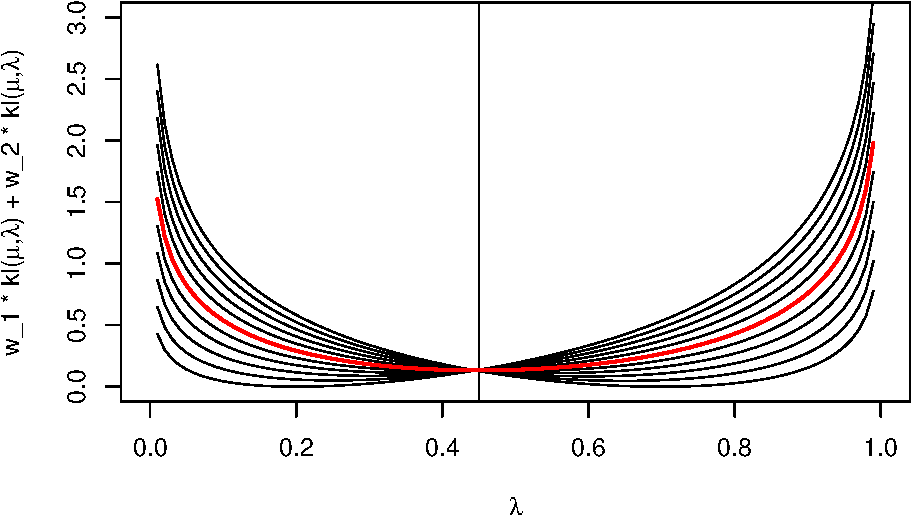
\includegraphics{kl_complexity_files/figure-latex/unnamed-chunk-1-1.pdf}

Given this general lower bound for the sampling complexity, or expected
number of draws, it makes sense to define the complexity of a Top-\(m\)
bandit problem using the Kullback-Leibler divergence. After all, besides
the number of arms and the experimenter-chosen confidence, it is just
how close arms are with respect to each other in terms of
Kullback-Leibler divergence that influences the sampling complexity. And
in general, a problem requiring more samples is of course considered to
be more complex (at least with respect to the samples, which is what
needs to be optimized).

Thus, following Kaufmann et al. (2016), define the complexity
\(\mathcal{K}_C(\nu)\) for the fixed confidence setting as

\begin{equation}
\mathcal{K}_C(\nu) = \inf_{A \, \text{PAC}} \lim_{\delta \to 0} \sup \frac{\mathbb{E}_{\nu}[\tau_{\delta}]}{\log \frac{1}{\delta}}.
\end{equation}

So if we were to plug in the lower bound on the sampling complexity, we
would arrive at a complexity measure that basically depends only on the
Kullback-Leibler measuring for each arm how far it is away from the
border between the two groups of arms. To see this, consider the lower
bound on the complexity measure given in Kaufmann et al. (2016):

\begin{equation*}
\mathcal{K}_C(\nu) \geq \sum_{a \in \mathcal{S}_m^*} \frac{1}{\KL(\nu_a, \nu_{[m+1]})} + \sum_{a \notin \mathcal{S}_m^*} \frac{1}{\KL(\nu_a, \nu_{[m]})}
\end{equation*}

Given this description, we can already note that an intuitive extension
of this complexity notion to the thresholding bandit problem might
involve replacing \(\mu_{[m]}\) and \(\mu_{[m+1]}\) by the actual
threshold \(\tau\) (notation in Locatelli et al.) that divides the group
above the threshold from the group below the threshold. In that case,
the previously used \(\alpha\) might be very similar to the \(\epsilon\)
used in Locatelli et al. (2016).

To get there, however, at least two important steps remain. First, we
need to define a complexity for the fixed budget problem. Second, we
need to create algorithms that can match the lower bound.

Kaufmann et al. are able to provide a bound on their complexity measure
in the fixed budget case, however only in the case of \textbf{two-armed}
bandit models. As demanded in their paper, a fixed-budget algorithm is
called consistent if the failure probability
\(p_t(\nu) := \mathbb{P}_{\nu}(\hat{S}_m \neq S^*_m)\) tends to zero as
the number of samples goes to infinity. Also, define the complexity in
the fixed-budget setting as follows:

\begin{equation}
\mathcal{K}_B(\nu) = \inf_{A \, \text{consistent}} \big(\lim_{t \to \infty} \sup - \frac{1}{t} \log p_t(\nu)\big)^{-1}.
\end{equation}

Given this definition, one can interpret the bound given in Theorem 12
of Kaufmann et al. directly as a lower bound on the complexity
\(\mathcal{K}_B(\nu)\) (note the inverse).

\begin{theorem}[Kaufmann et al., 2016] \label{theorem:KaufmannEtAlTheorem12}
Let $\nu = (\nu_1, \nu_2)$ be a two-armed bandit model such that $\mu_1 > \mu_2$. In the fixed-budget setting, any consistent algorithm satisfies:

\begin{equation*}
\lim_{t \to \infty} \sup - \frac{1}{t} \log p_t(\nu) \leq \inf_{(\nu_1', \nu_2') \in \mathcal{M}: \mu_1' < \mu_2'} \frac{\KL(\nu_1', \nu_1) + \KL(\nu_2', \nu_2)}{2}
\end{equation*}
\end{theorem}

For a proof, consider first the two different bandit models, \(\nu\) and
\(\nu'\), where we fix without loss of generality that \(a^* = 1\) is
the best arm in \(\nu\), while \(a^* = 2\) in \(\nu'\). Note that in
this case we don't necessarily try to fool the algorithm by a change of
distribution. Indeed, we want the algorithm \(\mathcal{A}\) to be
consistent for both problems. Since we are in the fixed-budget setting,
the stopping time is fixed at \(\tau = t\). Even though the correct
decision differs between the two problems, we focus on the event
\(A = (\hat{S}_1 = 1)\). Given the formulation in Kaufmann et al.
(2016), we have \(A \in \mathcal{F}_t = \mathcal{F}_{\tau}\). Now, we
can apply Lemma 1 as before, as it in essense gives a measure of how
different two bandit models are. Here, we want to know how different
\(\nu\) is from \(\nu'\), and so, given we have only two arms,

\begin{equation*}
\mathbb{E}_{\nu'}[N_1(t)]\KL(\nu_1', \nu_1) + \mathbb{E}_{\nu'}[N_2(t)]\KL(\nu_2', \nu_2) \geq \der(\mathbb{P}_{\nu'}(A),\mathbb{P}_{\nu}(A)))
\end{equation*}

The expectations were chosen with respect to \(\nu'\) in order to allow
the for the following: We have \(p_t(\nu) = 1 - \mathbb{P}_{\nu}(A)\)
and \(p_t(\nu') = \mathbb{P}_{\nu'}(A)\) (since \(A\) is wrong in
\(\nu'\)). But since algorithm \(\mathcal{A}\) is consistent for both
\(\nu\) and \(\nu'\), we know that there should exist some number of
samples such that the probability of event \(A\) is bigger in setting
\(\nu\) (where it is the correct decision), than in setting \(\nu'\)
(where this would be a wrong decision and failure). Thus, for every
\(\epsilon > 0\), there exists \(t_0(\epsilon)\) such that for all
\(t \geq t_0(\epsilon)\),
\(\mathbb{\nu'}(A) \leq \epsilon \leq \mathbb{P}_\nu(A)\). Consequently,
if we plug in the bound of \(\epsilon\) for \(\mathbb{P}_{\nu'}(A)\),
then

\begin{align*}
\mathbb{E}_{\nu'}[N_1(t)]\KL(\nu_1', \nu_1) + \mathbb{E}_{\nu'}[N_2(t)]\KL(\nu_2', \nu_2) & \geq \der(\epsilon,1-p_t(\nu))) \\
& = \epsilon \log \frac{\epsilon}{1-p_t(\nu)} + (1-\epsilon) \log \frac{1-\epsilon}{p_t(\nu)} \\
& \geq (1-\epsilon) \log \frac{1-\epsilon}{p_t(\nu)} + \epsilon \log \epsilon.
\end{align*}

Let \(\epsilon\) go to zero so that

\begin{align*}
\mathbb{E}_{\nu'}[N_1(t)]\KL(\nu_1', \nu_1) + \mathbb{E}_{\nu'}[N_2(t)]\KL(\nu_2', \nu_2)
& \geq \log \frac{1}{p_t(\nu)} = -\log p_t(\nu).
\end{align*}

Dividing both sides by \(t\) and taking the limsup, we arrive at

\begin{align*}
\lim_{t \to 0} \sup - \frac{1}{t} \log p_t(\nu)
& \leq \lim_{t \to 0} \sup \frac{1}{t} \sum_{a=1}^2 \mathbb{E}_{\nu'}[N_a(t)] \KL(\nu_a', \nu_a) \\
& \leq \max_{a=1,2} \KL(\nu_a', \nu_a),
\end{align*}

where the last line follows from the fact that the
\(\frac{1}{t} \sum_{a=1}^2 \mathbb{E}_{\nu'}[N_a(t)]\) part creates a
weighted average of the two divergences \(\KL(\nu_a', \nu_a)\). As noted
in Kaufmann et al. (2016), one arrives at the final result by choosing
\(\mu_1'\), \(\mu_2'\) so that
\(| \KL(\nu_1', \nu_1) - \KL(\nu_2', \nu_2) |\) is as small as possible.

Note that while deriving the lower bound on the complexity measure, we
have also derived the following lower bound on the failure probability
for the two-armed fixed-budget bandit:

\begin{equation*}
p_t(\nu) \geq \exp \big(- \sum_{a=1}^2 \mathbb{E}_{\nu'}[N_a(t)] \KL(\nu_a', \nu_a) \big)
\end{equation*}

or, to not rely on the share of samples attributed to each arm,

\begin{equation*}
p_t(\nu) \geq \exp \big(- \max_{a=1,2} \KL(\nu_a', \nu_a) \big).
\end{equation*}

\textbf{Mention something about the fact that we were not able to do
this for more than 2 arms and top-m bandits. How could it be extended to
that? How could it be extended to the threshold bandit?}

As noted by Kaufmann et al. (2016), the advantage of this lower bound is
that it makes the complexity in the fixed-confidence and the
fixed-budget setting directly comparable. The disadvantage of course
being that the result only holds for two-armed models. While the authors
were not able to derive directly comparable lower bounds for the
Top-\(m\) case, they did derive a first lower bound in the Gaussian case
with equal variances. While we would like to move beyond Gaussian
distributions in the work at hand, the idea for the proof might show a
way of how the ideas can be transferred to the thresholding bandit
problem. We first state the result and then discuss the proof.

\begin{lemma}[Lemma 15, Kaufmann et al., 2016] \label{theorem:KaufmannEtAlLemma15}
Let $\nu$ and $\nu'$ be two bandit models such that $S^*_m(\nu) \neq S*_m(\nu')$. Then

\begin{equation*}
\max \big( \mathbb{P}_{\nu}(S \neq S^*_m(\nu)), \mathbb{P}_{\nu'}(S \neq S^*_m(\nu')) \big) \geq \frac{1}{4} \exp \Big(-\sum_{a=1}^{K} \mathbb{E}_{\nu}[N_a] \KL(\nu_a, \nu_a') \Big).
\end{equation*}
\end{lemma}

The following theorem only holds in the case of Gaussian bandit models
with equal known variance.

\begin{theorem}[Theorem 17, Kaufmann et al., 2016] \label{theorem:KaufmannEtAlTheorem17}

Let $\mathcal{M}_m = \{\nu = (\nu_1, \dots, \nu_K): \nu_a = \mathcal{N}(\mu_a, \sigma^2), \mu_a \in \mathbb{R}, \mu_{[m]}\neq \mu_{[m+1]}\}.$ Furthermore, let $\nu$ be such that $\mu_1 > \dots > \mu_m > \mu_{m+1} > \dots > \mu_K$, and let

\begin{equation*}
H +(\nu) = \sum_{a=1}^m \frac{2\sigma^2}{(\mu_a - \mu_{m+1})^2}, \quad H^-(\nu) = \sum_{a=m+1}^K \frac{2\sigma^2}{(\mu_m - \mu_a)^2} \quad
and \quad
H(\nu) = H^+(\nu) + H^-(\nu).
\end{equation*}

There exists $a \in {1, \dots, m}$ and $b \in \{m+1, \dots, K\}$ such that the bandit model $\nu^{[a,b]}$ described in Figure 4 (Kaufmann et al., 2016) satisfies $H(\nu^{[a,b]}) < H(\nu)$ and is such that

\begin{equation*}
\max \big( p_t(\nu),p_t(\nu^{[a,b]})\big) \geq \frac{1}{4} \exp \big(-\frac{4t}{\bar{H}(\nu)}\big), \quad where \quad \bar{H}(\nu) = \frac{H(\nu) \min(H^+(\nu),H^-(\nu))}{H(\nu)+\min(H^+(\nu),H^-(\nu))}
\end{equation*}
\end{theorem}

Given that we are again in the Top-\(m\) setting, the proof idea is
similar to the proof of Theorem \ref{theorem:KaufmannEtAlTheorem4} in
that we again consider problems where we switch arms around the limit
seperating the two groups of arms as given implicitly by \(\mu_{[m]}\)
and \(\mu_{[m+1]}\). The hope here being that these methods could be
applied to the thresholding bandit problem where the threshold of course
gives the limit between the arms above and below the threshold. As we
have seen in chapter 1, this flip around the threshold was of course
used in the proof of the lower bound in Theorem 1 of Locatelli et al.
(2016). However, there, again, the distributions were assumed to be
Gaussian. This brings the big advantage that the Kullback-Leibler
divergence becomes symmetric, and the feedback can take values on all
\(\mathbb{R}\). And by using the complexity measure \(H(\nu)\), it is
also clear that there exists an arm that is undersampled with respect to
its contribution to the overall complexity of the problem (or sampled
exactly according to its contribution), which leads to leads to a
convenient upper bound on this arms number of draws which is again
employed in both the proof of Theorem
\ref{theorem:KaufmannEtAlTheorem17} and in Locatelli et al. (2016). It
is not clear yet, whether the same can also be done with other
complexity measures.

We do not repeat the proof here for now.

See p20!

What remains is to present algorithms that are able to match the lower
bounds derived so far.

\paragraph{Matching algorithm
strategies}\label{matching-algorithm-strategies}

Given those lower bounds, all that is left is to find algorithms which
are able to match the complexity. Sadly, not straightforward for
Bernoullis.

Kaufmann et al. (2016) do not present algorithms matching the lower
bound of Theorem \ref{theorem:KaufmannEtAlTheorem17}. They do consider
algorithms that connect to Theorem \ref{theorem:KaufmannEtAlTheorem4}
and Theorem \ref{theorem:KaufmannEtAlTheorem12}.

Given that Locatelli et al. (2016), and thus the problem we mostly
consider in this thesis, is in the fixed-budget setting, we are most
interested in the matching strategies for Theorem
\ref{theorem:KaufmannEtAlTheorem12}. However, given that the lower bound
applies only to two-armed bandits, the algorithms are of limited
practical interest. Furthermore, the algorithms proposed require
knowledge that is in general not available upfront.

For the example of Gaussian distributions, the knowledge of the
(potentially different) variance is assumed which enables a strategy
that pulls each arm proportional to its variance.

Even worse is the case of Bernoulli two-armed bandit models where the
proposed algorithm requires knowledge about the true parameters of the
distributions. That this limits the practical interest is also noted by
the authors of Kaufmann et al. (2016). Thus, they suggest to use uniform
sampling strategies in the case of two-armed Bernoulli bandits, and show
that there is not much to be lost by doing so.

Thus, Kaufmann et al. (2016) join a number of other papers like Audibert
et al. (2010) and Kaufmann and Kalyanakrishnan (2013) which struggle to
find matching strategies in the fixed-budget setting that do not rely on
knowledge of parameters or the complexity of the problem.

In contrast, Kaufmann et al. (2016) are able to show that their
complexity measure derived for the fixed-confidence setting,
\(\mathcal{K}_C(\nu)\), can be upper-bounded using the upper bound of
the sample complexity (number of pulls) given for the KL-LUCB algorithm
in Kaufmann and Kalyanakrishnan (2013). Consequently, in the case of
exponential family bandits, the complexity \(\mathcal{K}_C(\nu)\) is
bounded as given in equation (6) in Kaufmann et al. (2016):

\begin{equation*}
\sum_{a \in S^*_m} \frac{1}{K(\theta_a, \theta_{[m+1]})} + \sum_{a \notin S^*_m} \frac{1}{K(\theta_a,\theta_{[m]})} \leq \mathcal{K}_C(\nu) \leq 24 \min_{\theta \in [\theta_{[m+1]},\theta_{[m]}]} \sum_{a=1}^{K} \frac{1}{K^*(\theta_a, \theta)},
\end{equation*}

where \(K(\theta, \theta') = \KL(\nu_{\theta}, \nu_{\theta'})\) for
\((\theta, \theta') \in \Theta^2\) was defined as the shorthand for the
Kullback-Leibler divergence for two distributions from the exponential
family parameterized by \(\theta\) and \(\theta'\) respectively.
\(K^*(\theta,\theta') = K(\theta^*, \theta)\) is the Chernoff
distribution between the two distributions, where \(\theta^*\) is chosen
so that \(K(\theta^*,\theta) = K(\theta^*, \theta')\).

\subsubsection{Optimal Best Arm
Identification}\label{optimal-best-arm-identification}

A very similar application of the KL divergence has been given in
Garivier and Kaufmann to derive a lower bound on the sample complexity
in the case of best arm identification. In particular, the
transportation Lemma 1 is used again. And a matching algorithm for
\(K \geq 2\) arms is proposed.

Talk about: - Not a simple sum of squares - Idea of algorithm: Equalize
the probability of all wrong decisions

In Garivier and Kaufmann (2016), the authors are able to derive a
somewhat similar lower bound on the sample complexity of a \(K\)-armed
bandit in the single best arm identification problem with fixed
confidence. Additionally, they provide a \(\delta\)-PAC algorithm
achieving said bound asymptotically.

In particular, the authors pick up Lemma 1 from Kaufmann et al. (2016)
-- which we discussed above -- to derive the lower bound. While
presenting these results, we try to stick as much as possible with the
notation used so far. In particular, we let for distributions
\(\nu_{\theta}\) from a canonical exponential family, which can be
parameterized by its mean \(\stackrel{.}{b}(\theta) = \mu\) and thus be
written as \(\nu^{\mu}\); for these, we continue to write the
Kullback-Leibler divergence as

\begin{equation*}
\KL(\mu, \mu') = \KL(\nu^{\mu},\nu^{\mu'}) = \KL(\nu_{\theta},\nu_{\theta'}) = \KL(\nu, \nu')
\end{equation*}

while \(d(x,y)\) continues to represent the binary relative entropy.

As we will consider only problems with exponential family distributions,
the distributions can be parameterized by their means. Therefore, if we
let \(\mathcal{S}\) to be a set of bandit models with \(K\)
distributions each, then each model is fully defined by a vector
\(\bm{\mu} = (\mu_1, \dots, \mu_K)\). Assume that every
\(\bm{\mu} \in \mathcal{S}\) has a unique maximum given by
\(a^*(\bm{\mu})\) such that
\(\mu_{a^*} > \max_{a \neq a^*(\bm{\mu})} \mu_a\). In order to fix the
confidence, we specify the risk \(\delta\). The strategies corresponding
to this risk are called \(\delta\)-PAC if for every
\(\bm{\mu} \in \mathcal{S}\),
\(\mathbb{P}_{\bm{\mu}}(\tau_{\delta} < \infty) = 1\) (the strategy ends
surely after a finite number of samples) and
\(\mathbb{P}_{\bm{\mu}}(\hat{a}_{\tau_{\delta}} \neq a^*) \leq \delta\)
(the probability of picking not the optimal arm is smaller than the
fixed risk). As in Garivier and Kaufmann (2016), we introduce the set of
problems for which the optimal arm is different from the one in
\(\bm{\mu}\):

\begin{equation*}
\text{Alt}(\bm{\mu}) := \{\bm{\lambda} \in \mathcal{S}: a^*(\bm{\lambda}) \neq a^*(\bm{\mu})\}
\end{equation*}

where \(\bm{\lambda}\) is the vector of means defining the distributions
of the alternative problem to \(\bm{\mu}\). Lastly, we have the set of
probability distributions on the arms \(\mathcal{A}\):
\(\Sigma_K = \{w \in \mathbb{R}_{+}^K: w_1 + \dots + w_K = 1\}\).
\marginpar{Give more intuition for what these probability distributions are}
We are now ready to state the theorem.

\begin{theorem}[Theorem 1, Garivier and Kaufmann, 2016] \label{theorem:GarivierKaufmannTheorem1}
Let $\delta \in (0,1)$. For any $\delta$-PAC strategy and any bandit model $\bm{\mu} \in \mathcal{S}$,

\begin{equation*}
\mathbb{E}_{\bm{\mu}} [\tau_{\delta}] \geq T^*(\bm{\mu}) \text{\em{d}}(\delta,1-\delta),
\end{equation*}

where 

\begin{equation} \label{eq:GarivierKaufmann_Theorem1_Game}
T^*(\bm{\mu})^{-1} := \sup_{w \in \Sigma_K} \inf_{\bm{\lambda} \in \text{\em{Alt}}(\bm{\mu})} \left( \sum_{a=1}^K w_a \text{\em{KL}}(\mu_a, \lambda_a)\right) .
\end{equation}
\end{theorem}

And so we see that the two bounds on the sample complexity (one for
Top-\(m\), one for best arm identification) differ only in the way that
they build the sum of Kullback-Leibler divergences over the \(K\) arms.
In contrast to Theorem \ref{theorem:KaufmannEtAl2016Theorem1}, here the
contribution of each arm through its KL-divergence is weighted. The
difference is that while we were able to very clearly describe the
change of distribution in the Top-\(m\) case for each arm -- for each
arm, we specified an alternative model that yields a new set of \(m\)
optimal arms -- we now consider all alternative models that yield a
different best arm than the model \(\bm{\mu}\). In the previous theorem,
we sum over the complexity of each individual arm, as the change in
distribution only ever touches one arm, thus leading to a KL-divergence
of 0 for the other arms while still changing the optimal set. Here, we
consider all instances of alternative models \(\bm{\lambda}\), and thus
also those in which several arms are modified (and thus have a
KL-divergence unequal 0 in the result of Lemma 1).

\emph{Proof of Theorem \ref{theorem:GarivierKaufmannTheorem1}}: As
stated before, we let \(\delta \in (0,1)\),
\(\bm{\mu} \in \mathcal{S}\), and only consider \(\delta\)-PAC
strategies. As before, \(N_a(t)\) describes the random number of pulls
of arm \(a\) until time \(t\), for all \(t\geq 1\). Again, Lemma
\ref{theorem:KaufmannEtAlLemma1} states how the failure probability
\(\delta\) relates to the expected number of draws of each arm given two
models which differ in their optimal arm, and where it is evaluated
based on the Kullback-Leibler divergence for each pair of arms how much
the two models differ:

\begin{equation*}
\forall \lambda \in \mathcal{S}: a^*(\lambda) \neq a^*(\mu), \sum_{a=1}^K \KL(\mu_a,\lambda_a)\mathbb{E}_{\bm{\mu}}[N_a(\tau_{\delta})] \geq \d(\delta, 1- \delta).
\end{equation*}

As mentioned, we now do not consider a specific alternative for each
arm, but instead look at the infimum over all the possible alternatives,
and use the fact that
\(\mathbb{E}_{\bm{\mu}}[\tau_{\delta}] = \sum_{a=1}^K \mathbb{E}_{\bm{\mu}}[N_a(\tau_{\delta})]\):

\begin{align*}
\der(\delta, 1-\delta) & \leq \inf_{\lambda \in \text{Alt}(\bm{\mu})} \mathbb{E}_{\bm{\mu}}[\tau_{\delta}] \Big(\sum_{a=1}^K \frac{\mathbb{E}_{\bm{\mu}}[N_a]}{\mathbb{E}_{\mu}[\tau_{\delta}]} \KL(\mu_a, \lambda_a)\Big) \\
& = \mathbb{E}_{\bm{\mu}}[\tau_{\delta}] \inf_{\lambda \in \text{Alt}(\bm{\mu})} \Big(\sum_{a=1}^K \frac{\mathbb{E}_{\bm{\mu}}[N_a]}{\mathbb{E}_{\mu}[\tau_{\delta}]} \KL(\mu_a, \lambda_a)\Big) \\
& \leq \mathbb{E}_{\bm{\mu}}[\tau_{\delta}] \sup_{w \in \Sigma_K} \inf_{\lambda \in \text{Alt}(\bm{\mu})} \Big(\sum_{a=1}^K w_a \KL(\mu_a, \lambda_a)\Big).
\end{align*}

As stated in Garivier and Kaufmann (2016), the term
\(\frac{\mathbb{E}_{\bm{\mu}}[N_a]}{\mathbb{E}_{\mu}[\tau_{\delta}]}\)
gives the fraction of draws each arm receives. This value, however,
depends on the used algorithm. To make it hold for any \(\delta\)-PAC
algorithm, it is replaced by the supremum over \(\Sigma_K\), which is
the distribution over these fractions for any \(\mathcal{A}\), that is,
for any \(\delta\)-PAC strategy.

This lower bound can be interpreted as a Minimax game, where the
experimenter has to choose the share of samples he attributes to each
arm in a way that is optimal given that nature will respond and choose
the most difficult alternative model given his weights. Thus, to make
the lower bound practical, it is a matter of finding the optimal weights
\(w^*(\bm{\mu})\). This step did not occur in the previous lower bound,
as the alternative models were made specific by changing the
distribution of one arm with respect to the ``border'' between the two
groups of arms.

In any case, the existence of the optimal weights suggests an algorithm
that keeps track of the share of samples that is attributed to each arm
and makes sure that it stays close to the optimum until some decision
rule assures that the \(\delta\)-PAC condition is fulfilled.

And so by assuring the reader that there are ways to compute \(w_a^*\)
and \(T^*\) given \(\bm{\mu}\) (see chapter 2.2 in Garivier and Kaufmann
(2016)), we can now introduce the \emph{Track-and-Stop} strategy given
in Garivier and Kaufmann (2016) that is able to match the lower bound by
the intuition given above.

When going from theory to algorithm, the obvious problem is of course
that we do no longer know \(\bm{\mu}\) and thus cannot simply calculate
the optimal weights. Instead, we are estimating the maximum likelihood
estimates \(\hat{\mu}(t) = (\hat{\mu}_1(t), \dots, \hat{\mu}_K(t))\) of
the true mean at the current round \(t\) and need to base our weights
based on these. It is however problematic to rely on these sample means
as we are inherently unsure about them. And so wrong estimates, which
naturally occur most easily in the beginning when not many samples have
been pulled, are prone to lead to wrong weights. Thus, if a wrong
estimate \(\hat{\mu}_a\) for arm \(a\) leads to a small weight \(w_a\),
then neither the estimate nor the weight will be correct soon. Thus,
Kaufmann and Garivier conclude that ``a naive plug-in sampling rule
sometimes fails''. They propose to enforce a certain minimum level of
exploration to make sure that arms that erroneously received a very
small weight will be further explored regardless.

A very intuitive fix to this problem is the solution proposed in Lemma 8
of Garivier and Kaufmann (2016), with their \(D-Tracking\) rule.
Basically, whenever an arm has received a very low number of pulls
\(N_a(t)\) given the number of iterations so far, \(t\) and the number
of arms \(K\) that have to share the samples, pull the arm that has
received the smallest amount of samples so far. Else, pull the arm which
number of pulls so far \(N_a(t)\) is the furthest away from what its
optimal share \(t\cdot w^*_a(\hat{\bm{\mu}}(t))\) would be. Given this
sampling rule, the authors can show in their Proposition 9 that the
empirical proportion of draws converges in probability to the optimal
weights given the true means.

When combining this sampling rule with an appropriate stopping rule, the
authors are able to prove in Theorem 14 an upper bound on the expected
sampling complexity \(\mathbb{E}_{\mu}[\tau_{\delta}]\). The stopping
rule ensures that the algorithm explores sufficiently to promise a risk
smaller than \(\delta\), while stopping as soon as possible. Given that
the sampling rule is independent of this stopping rule, the rule boils
down to a statistical test at every iteration and thus is a sequential
test based on the current estimate of \(\hat{\bm{\mu}}\). The Chernoff's
Stopping Rule proposed in Garivier and Kaufmann (2016) calculates for
each arm \(a\in \mathcal{A}\) the Generalized Likelihood Ratio statistic
with every arm \(b \in \mathcal{A}^{\setminus a}\), which for
\(\hat{\mu}_a(t) \geq \hat{\mu}_b(t)\) can be written as

\begin{equation*}
Z_{a,b}(t) = - Z_{b,a} = N_a(t) \KL(\hat{\mu},\hat{\mu}_{a,b})) + N_b(t) \KL(\hat{\mu}_{b(t)}, \hat{\mu}_{a,b}),
\end{equation*}

where

\begin{equation*}
\hat{\mu}_{a,b}(t) := \frac{N_a(t)}{N_a(t) + N_b(t)}\hat{\mu}_a + \frac{N_b(t)}{N_a(t) + N_b(t)}\hat{\mu}_b.
\end{equation*}

Consequently, a sensible idea for a stopping rule would be that there
has to be an arm \(a \in \mathcal{A}\) for which
\(Z_{a,b} \geq 0 \forall b \in \mathcal{A}^{\setminus a}\) (which is
always fulfilled if there is a uniquely best arm), and, additionally, we
demand that for this arm the smallest of the \((K-1)\) test statistics
has to be larger than an exploration threshold \(\beta(t, \delta)\).
Consequently, the final number of samples \(\tau_{\delta}\) of an
algorithm is given by:

\begin{equation*}
\tau_{\delta} = \inf \{t \in \mathbb{N}: \exists a \in \mathcal{A}, \forall b\in \mathcal{A}^{\setminus a}, Z_{a,b}(t) > \beta(t, \delta)\}
\end{equation*}

Demanding that the optimal exploration threshold increases in rounds
\(t\) (if we have more samples, require more certainty; also, punish for
failing previous tests) and decreases in the risk \(\delta\), and does
so at a diminishing rate, the optimal threshold derived in Theorem 10 of
Garivier and Kaufmann (2016) makes sense intuitively:

\begin{equation*}
\beta(t, \delta) = \log \Big(\frac{2t(K-1)}{\delta}\Big)
\end{equation*}

.


\end{document}
